\section{Implications for Distributed Systems}

\subsection{Space is simply time}

Dedalus programs can model many classes of distributed systems.  Take the (distributed) program

\begin{Dedalus}
ping(@A, B)@N + r(A, B) \(\leftarrow\)
  init(A, B)@N; 

pong(@B, A)@N + r(A, B) \(\leftarrow\)
  ping(@A, B)
\end{Dedalus}

We may regard  \emph{r()} as a function over the attributes occurring in the body of the rule.  The implementation or \emph{r()} is provided by
the model.  For example:

\subsubsection{Synchronous Systems}

r(\_) = 1 for all \_.  Computation proceeds in rounds.

\subsubsection{Asynchronous Systems}

The return value of r may be any arbitrary integer, positive or negative, including a NULL integer indicating an infinite value.

\subsubsection{Lamport Clocks}

As a middle ground, we might wish to enforce a constraint that $r(\_) > 0$.  Doing so would entail implementing a \emph{Lamport Clock}.

\begin{figure}[t]
  \centering
  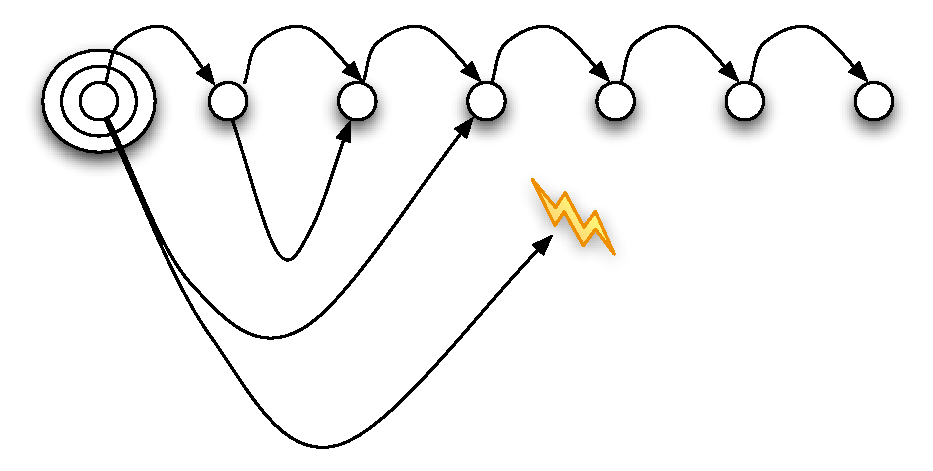
\includegraphics[width=0.75\linewidth]{dedalus-time.pdf}
  \label{fig:dedalus-time}
  \caption{Time moves forward in three ways: across strata, to the next fixpoint, and to some future fixpoint.}
\vspace{-8pt}
\end{figure}



\subsection{Dedalus Programs can be efficiently implemented}

:)

\subsubsection{Local stratification on time}

\subsubsection{Time is infinite but punctuated}

and indeed, so are any input streams.  we may dequeue as many events as we like from a given stream by using the mapping
between the elements in the queue and the time relation.  in the simplest case this mapping would be from the ordering domain 
of the queue to the time domain, but we can establish more complicated data-dependent mappings by including other attributes 
(e.g. we could implement QoS by including the address in the mapping and dequeueing a different number of items per host
per time unit).
